\documentclass[a4paper, 12pt]{article}

\usepackage{graphicx}
\usepackage{longtable}
\graphicspath{ {images/} }

\newcommand{\templates}{../../template}
\usepackage[a4paper, margin=2.5cm]{geometry}

\usepackage{enumitem}
\setlist[itemize]{noitemsep}
\setlist[enumerate]{noitemsep}

\let\oldpar\paragraph
\renewcommand{\paragraph}[1]{\oldpar{#1\\}\noindent}
\usepackage{graphicx}
\usepackage{hyperref}
\usepackage{makecell}

\newcommand{\settitolo}[1]{\newcommand{\titolo}{#1\\}}
\newcommand{\setprogetto}[1]{\newcommand{\progetto}{#1\\}}
\newcommand{\setcommittenti}[1]{\newcommand{\committenti}{#1\\}}
\newcommand{\setredattori}[1]{\newcommand{\redattori}{#1\\}}
\newcommand{\setrevisori}[1]{\newcommand{\revisori}{#1\\}}
\newcommand{\setresponsabili}[1]{\newcommand{\responsabili}{#1\\}}
\newcommand{\setversione}[1]{
	\ifdefined\versione\renewcommand{\versione}{#1\\}
	\else\newcommand{\versione}{#1\\}\fi
}
\newcommand{\setdestuso}[1]{\newcommand{\uso}{#1\\}}
\newcommand{\setdescrizione}[1]{\newcommand{\descrizione}{#1\\}}

\newcommand{\makefrontpage}{
	\begin{titlepage}
		\begin{center}

		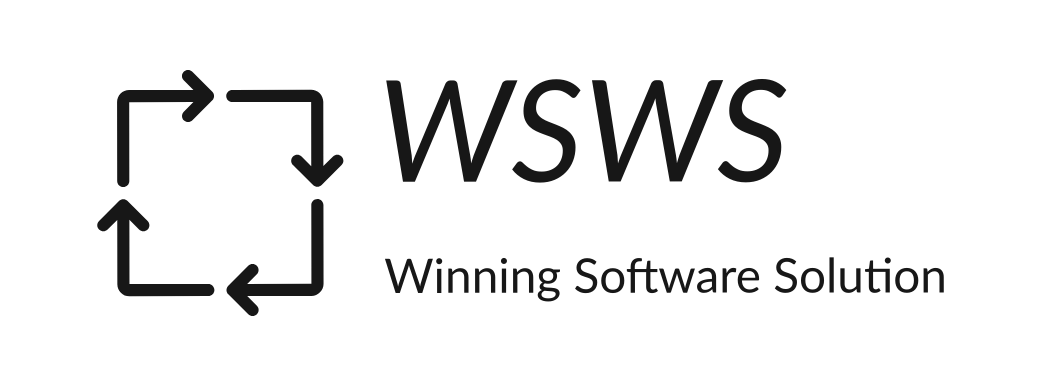
\includegraphics[width=0.4\textwidth]{../../template/WSWS-logos_transparent_crop}\\

		{\Large Winning Software Solution}\\[6pt]
		\href{mailto://winningsoftwaresolution@gmail.com}{winningsoftwaresolution@gmail.com}\\
		
		\ifdefined\progetto
		\vspace{1cm}
		{\Large\progetto}
		{\large\committenti}
		\else\fi
		
		\vspace{1.5cm}
		{\LARGE\titolo}
		
		\vfill
		
		\begin{tabular}{r | l}
		\multicolumn{2}{c}{\textit{Informazioni}}\\
		\hline
		
		\ifdefined\redattori
			\textit{Redattori} &
			\makecell[l]{\redattori}\\
		\else\fi
		\ifdefined\revisori
			\textit{Revisori} &
			\makecell[l]{\revisori}\\
		\else\fi
		\ifdefined\responsabili
			\textit{Respondabili} &
			\makecell[l]{\responsabili}\\
		\else\fi
		
		\ifdefined\versione
			\textit{Versione} & \versione
		\else\fi
		
		\textit{Uso} & \uso
		
		\end{tabular}
		
		\vspace{2cm}
		
		\ifdefined\descrizione
		Descrizione
		\vspace{6pt}
		\hrule
		\descrizione
		\else\fi
		\end{center}
	\end{titlepage}
}
\usepackage{hyperref}
\usepackage{array}
\usepackage{tabularx}

\def\vers#1-#2-#3-#4-#5\\{#1&#2&#3&#4&#5\\\hline}

\newcommand{\addversione}[5]{
	\ifdefined\versioni
		\let\old\versioni
		\renewcommand{\versioni}{#1&#2&#3&#4&#5\\\hline\old}
	\else
		\newcommand{\versioni}{#1&#2&#3&#4&#5\\\hline}
	\fi
}

\newcommand{\setversioni}[1]{\newcommand{\versioni}{#1}}

\newcommand{\makeversioni}{
	\begin{center}
		\begin{tabularx}{\textwidth}{|c|c|c|c|X|}
		\hline
		\textbf{Versione} & \textbf{Data} & \textbf{Persona} & \textbf{Attivtà} & \textbf{Descrizione} \\
		\hline
		\versioni
		\end{tabularx}
	\end{center}
	\clearpage
}

\settitolo{Analisi dei requisiti}
\setprogetto{ShopChain}
\setcommittenti{SyncLab}
\setredattori{Raffaele Oliviero}
\setdestuso{esterno}
\setdescrizione{
Lista Metodi
}

\addversione{0.0.0}{2/2/2022}{Raffaele Oliviero}{Redazione}{Strutturazione del documento}
\addversione{0.0.1}{4/3/2022}{Andrea Volpe}{Redazione}{Inserimento metodi pubblici}
\addversione{0.0.2}{5/3/2022}{Raffaele Oliviero}{Redazione}{Inserimento metodi pubblici e stesura \ref{tipi}}

\begin{document}

\makefrontpage

\makeversioni

\section{Introduzione}
\subsection{Scopo del documento}
Il documento elenca i metodi pubblici di ogni classe, descrivendone i loro parametri di invocazione, i loro return e il comportamento.

\section{Tipi usati frequentemente}\label{tipi}
Un breve elenco dei tipi comunemente usati e dei loro attributi

\subsection{paymentEntry}
Un \textbf{articolo} in vendita\\
\textbf{Parametri:}
\begin{itemize}
\item[\texttt{id}]	l'id dell'articolo
\item[\texttt{seller}] l'indirizzo del wallet del venditore
\item[\texttt{price}] il prezzo in centesimi di dollaro
\end{itemize}

\subsection{settledPayment}
Una \textbf{transazione}\\
\textbf{Parametri:}
\begin{itemize}
\item[\texttt{id}]	l'id della transazione
\item[\texttt{paymentEntryID}]	l'id dell'articolo acquistato
\item[\texttt{client}] l'indirizzo del wallet dell'acquirente
\item[\texttt{status}] lo stato della transazione con i seguenti significati:
	\begin{itemize}
	\item[\texttt{0}] la transazione è stata cancellata
	\item[\texttt{1}] la transazione è stata pagata
	\item[\texttt{2}] i fondi sono stati sbloccati
	\item[\texttt{3}] la transazione è timed out
	\end{itemize}
\item[\texttt{created}] la data dell'ultima modifica
\item[\texttt{confirmed}] se la transazione è stata chiusa, ne indica la data di chiusura
\end{itemize}

\subsection{payment}
Una \textbf{transazione} in cui sono contenute più informazioni\\
\textbf{Parametri:}
\begin{itemize}
\item[\texttt{id}] l'id della transazione
\item[\texttt{buyer}] l'indirizzo del wallet dell'acquirente
\item[\texttt{seller}] l'indirizzo del wallet del venditore
\item[\texttt{price}] il prezzo in centesimi di dollaro
\item[\texttt{status}] lo stato della transazione con i seguenti significati:
	\begin{itemize}
	\item[\texttt{0}] la transazione è stata cancellata
	\item[\texttt{1}] la transazione è stata pagata
	\item[\texttt{2}] i fondi sono stati sbloccati
	\item[\texttt{3}] la transazione è timed out
	\end{itemize}
\item[\texttt{created}] la data dell'ultima modifica
\item[\texttt{confirmed}] se la transazione è stata chiusa, ne indica la data di chiusura
\end{itemize}

\section{Lista dei metodi pubblici}
\subsection{Persistence}
class Persistence
\subsubsection{constructor(sql, shopContract)}
Crea ShopContractEventManager\\
\textbf{Parametri}\\
sql: SQL\_Interface\\
shopContract: ShopContract\_Interface
\subsubsection{getPaymentByBuyer(buyer): Promise$<$payment[ ]$>$}
Restituisce le transazioni il cui acquirente corrisponde a \texttt{buyer}\\
\textbf{Parametri}\\
buyer: string\\
\textbf{Valore Restituito}\\
Promise$<$payment[ ]$>$
\subsubsection{getPaymentBySeller(seller): Promise$<$payment[ ]$>$}
Restituisce le transazioni il cui venditore corrisponde a \texttt{buyer}\\
\textbf{Parametri}\\
seller: string\\
\textbf{Valore Restituito}\\
Promise$<$payment[ ]$>$
\subsubsection{getPaymentEntryByID(id): Promise$<$paymentEntry$>$}
Restituisce il prodotto identificato da \texttt{id}\\
\textbf{Parametri}\\
id: bigint\\
\textbf{Valore Restituito}\\
Promise$<$paymentEntry$>$
\subsubsection{getPaymentByID(id): Promise$<$payment$>$}
Restituisce la transazione identificata da \texttt{id}\\
\textbf{Parametri}\\
id: bigint\\
\textbf{Valore Restituito}\\
Promise$<$payment$>$

\subsection{ServerManager}
class ServerManager
\subsubsection{setContract(shopContract) : ServerManager}
Imposta un contratto\\
\textbf{Parametri}\\
shopContract : ShopContract\_Interface\\
\textbf{Valore Restituito}\\
%\underline{\href{\linkServerManager}{ServerManager}}\\
ServerManager\\
\subsubsection{setSQL(sql) : ServerManager}
Imposta una connessione SQL\\
\textbf{Parametri}\\
sql : SQL\_Interface\\
\textbf{Valore Restituito}\\
ServerManager
\subsubsection{setPageCreator(page): ServerManager}
Imposta un PageCreator\\
\textbf{Parametri}\\
page : PageCreator\\
\textbf{Valore Restituito}\\
ServerManager
\subsubsection{start() : ServerManager}
Crea e avvia un nuovo server\\
\textbf{Parametri}\\
\textbf{Valore Restituito}\\
ServerManager\\
\textbf{Eccezioni}\\
AssertionError?
\subsubsection{closeServer() : void}
Chiude la connessione con il server\\
\textbf{Parametri}\\
\textbf{Valore Restituito}\\
void

\subsection{SQL\_Interface}
interface SQL\_Interface
\subsubsection{insertPaymentEntry(entry): Promise$<$void$>$}
Inserisce un nuovo prodotto nel database\\
\textbf{Parametri}\\
entry: paymentEntry\\
\textbf{Valore Restituito}\\
Promise$<$void$>$
\subsubsection{insertSettledPayment(entry): Promise$<$void$>$}
Inserisce un nuovo pagamento nel database\\
\textbf{Parametri}\\
entry: settledPayment\\
\textbf{Valore Restituito}\\
Promise$<$void$>$
\subsubsection{updateSettledPayment(id, status, timestamp): Promise$<$void$>$}
Aggiorna un pagamento nel database\\
\textbf{Parametri}\\
id: bigint,\\ 
status: number,\\
timestamp: bigint\\
\textbf{Valore Restituito}\\
Promise$<$void$>$
\subsubsection{getPaymentByBuyer(buyer): Promise$<$payment[ ]$>$}
Restituisce i pagamenti di uno specifico acquirente\\
\textbf{Parametri}\\
buyer: string\\
\textbf{Valore Restituito}\\
Promise$<$payment[ ]$>$
\subsubsection{getPaymentBySeller(seller): Promise$<$payment[ ]$>$}
Restituisce i pagamenti di uno specifico venditore\\
\textbf{Parametri}\\
seller: string\\
\textbf{Valore Restituito}\\
Promise$<$payment[ ]$>$
\subsubsection{getPaymentEntryByID(id): Promise$<$paymentEntry$>$}
Restituisce uno specifico prodotto\\
\textbf{Parametri}\\
id: bigint\\
\textbf{Valore Restituito}\\
Promise$<$paymentEntry$>$
\subsubsection{getPaymentByID(id): Promise$<$payment$>$}
Restituisce uno specifico pagamento\\
\textbf{Parametri}\\
id: bigint\\
\textbf{Valore Restituito}\\
Promise$<$payment$>$
\subsubsection{getLastSyncBlock(): Promise$<$number$>$}
Restituisce l'ultimo blocco sincronizzato\\
\textbf{Parametri}\\
\textbf{Valore Restituito}\\
Promise$<$number$>$
\subsubsection{setLastSyncBlock(block): Promise $<$void$>$}
Imposta l'ultimo blocco sincronizzato al valore passato come parametro\\
\textbf{Parametri}\\
block: number\\
\textbf{Valore Restituito}\\
Promise$<$void$>$

\subsection{SQL}
class SQL implements SQL\_Interface
\subsubsection{constructor()}
Effettua la connessione al DB usando le impostazioni contenute nel file \texttt{.env}\\
\subsubsection{closeConnection(): void}
Chiude la connessione con il database\\
\textbf{Parametri}\\
\textbf{Valore Restituito}\\
void
\subsubsection{insertPaymentEntry(entry): Promise$<$void$>$}
Inserisce un nuovo prodotto nel database\\
\textbf{Parametri}\\
entry: paymentEntry\\
\textbf{Valore Restituito}\\
Promise$<$void$>$
\subsubsection{insertSettledPayment(entry): Promise$<$void$>$}
Inserisce un nuovo pagamento nel database\\
\textbf{Parametri}\\
entry: settledPayment\\
\textbf{Valore Restituito}\\
Promise$<$void$>$
\subsubsection{updateSettledPayment(id, status, timestamp): Promise$<$void$>$}
Aggiorna un pagamento nel database\\
\textbf{Parametri}\\
id: bigint,\\ 
status: number,\\
timestamp: bigint\\
\textbf{Valore Restituito}\\
Promise$<$void$>$
\subsubsection{getPaymentByBuyer(buyer): Promise$<$payment[ ]$>$}
Restituisce i pagamenti di uno specifico acquirente\\
\textbf{Parametri}\\
buyer: string\\
\textbf{Valore Restituito}\\
Promise$<$payment[ ]$>$
\subsubsection{getPaymentBySeller(seller): Promise$<$payment[ ]$>$}
Restituisce i pagamenti di uno specifico venditore\\
\textbf{Parametri}\\
seller: string\\
\textbf{Valore Restituito}\\
Promise$<$payment[ ]$>$
\subsubsection{getPaymentEntryByID(id): Promise$<$paymentEntry$>$}
Restituisce uno specifico prodotto\\
\textbf{Parametri}\\
id: bigint\\
\textbf{Valore Restituito}\\
Promise$<$paymentEntry$>$
\subsubsection{getPaymentByID(id): Promise$<$payment$>$}
Restituisce uno specifico pagamento\\
\textbf{Parametri}\\
id: bigint\\
\textbf{Valore Restituito}\\
Promise$<$payment$>$
\subsubsection{getLastSyncBlock(): Promise$<$number$>$}
Restituisce l'ultimo blocco sincronizzato\\
\textbf{Parametri}\\
\textbf{Valore Restituito}\\
Promise$<$number$>$
\subsubsection{setLastSyncBlock(block): Promise $<$void$>$}
Imposta l'ultimo blocco sincronizzato al valore passato come parametro\\
\textbf{Parametri}\\
block: number\\
\textbf{Valore Restituito}\\
Promise$<$void$>$

\subsection{Server}
class Server
\subsubsection{constructor(db, page)}
Associa il database e il creatore di pagina e crea ed inizializza Express\\
\textbf{Parametri}\\
\subsubsection{close(): void}
Chiude la connessione con il server\\
\textbf{Parametri}\\
\textbf{Valore Restituito}\\
void

\subsection{PageCreator}
class PageCreator
\subsubsection{landPage(req, res, db): void} 
Renderizza e invia la pagina \texttt{landing page} al client\\
\textbf{Parametri}\\
req: Request,\\
res: Response,\\
db: Persistence\\
\textbf{Valore Restituito}\\
void
\subsubsection{helpPage(req, res): void}
Renderizza e invia la pagina \texttt{help} al client\\
\textbf{Parametri}\\
req: Request,\\
res: Response\\
\textbf{Valore Restituito}\\
void
\subsubsection{mainPage(req, res): void}
Renderizza e invia la pagina \texttt{principale} al client\\
\textbf{Parametri}\\
req: Request,\\
res: Response\\
\textbf{Valore Restituito}\\
void
\subsubsection{confirmPage(req, res, db): void}
Renderizza e invia la pagina \texttt{?} al client\\
\textbf{Parametri}\\
req: Request,\\
res: Response,\\
db: Persistence\\
\textbf{Valore Restituito}\\
void
\subsubsection{paymentByBuyerPage(req, res, db): void}
Renderizza e invia la pagina delle \texttt{transazioni effettuate} al client\\
\textbf{Parametri}\\
req: Request,\\
res: Response,\\
db: Persistence\\
\textbf{Valore Restituito}\\
void
\subsubsection{detailPage(req, res, db): void}
Renderizza e invia la pagina dei \texttt{dettagli transazione?} al client\\
\textbf{Parametri}\\
req: Request,\\
res: Response,\\
db: Persistence\\
\textbf{Valore Restituito}\\
void
\subsubsection{paymentBySellerPage(req, res, db): void}
Renderizza e invia la pagina delle \texttt{transazioni in ingresso} al client\\
\textbf{Parametri}\\
req: Request,\\
res: Response,\\
db: Persistence\\
\textbf{Valore Restituito}\\
void

\subsection{ShopContract\_Interface}
interface ShopContract\_Interface
\subsubsection{getBlockTime(block) : Promise$<$bigint$>$}
Restituisce il timestamp di \texttt{block}\\
\textbf{Parametri}\\
block: number\\
\subsubsection{addedPaymentEntry(options) : EventEmitter}
Emette un evento di articolo aggiunto\\
\textbf{Parametri}\\
options: pastEventOptions
\subsubsection{paymentSettled(options) : EventEmitter}
Emette un evento di transazione effettuata\\
\textbf{Parametri}\\
options: pastEventOptions
\subsubsection{statusChange(options) : EventEmitter}
Emette un evento di cambio di stato\\
\textbf{Parametri}\\
options: pastEventOptions
\subsubsection{getSettledPayment(id) : Promise$<$settledPayment$>$}
Restituisce la transazione corrispondente a \texttt{id}\\
\textbf{Parametri}\\
id: bigint
\subsubsection{getPaymentEntry(id) : Promise$<$settledPayment$>$}
Restituisce l'articolo in vendita corrispondente a \texttt{id}\\
\textbf{Parametri}\\
id: bigint

\subsection{ShopContract (typescript)}
ShopContract implementa ShopContract\_Interface
\subsubsection{constructor(web3)}
Associa web3 e il contratto\\
\textbf{Parametri}\\
web3: Web3\\
\subsubsection{getBlockTime(block) : Promise$<$bigint$>$}
Restituisce il timestamp di \texttt{block}\\
\textbf{Parametri}\\
block: number\\
\subsubsection{addedPaymentEntry(options) : EventEmitter}
Emette un evento di articolo aggiunto\\
\textbf{Parametri}\\
options: pastEventOptions
\subsubsection{paymentSettled(options) : EventEmitter}
Emette un evento di transazione effettuata\\
\textbf{Parametri}\\
options: pastEventOptions
\subsubsection{statusChange(options) : EventEmitter}
Emette un evento di cambio di stato\\
\textbf{Parametri}\\
options: pastEventOptions
\subsubsection{getSettledPayment(id) : Promise$<$settledPayment$>$}
Restituisce la transazione corrispondente a \texttt{id}\\
\textbf{Parametri}\\
id: bigint
\subsubsection{getPaymentEntry(id) : Promise$<$settledPayment$>$}
Restituisce l'articolo in vendita corrispondente a \texttt{id}\\
\textbf{Parametri}\\
id: bigint

\subsection{ShopContractEventManager}
ShopContract implementa ShopContract\_Interface
\subsubsection{contstructor(sql, shopContract)}
Crea la classe e associa gli eventi da ascoltare\\
\textbf{Parametri}\\
sql: SQL\_Interface
shopContract: ShopContract\_Interface
 
\subsection{ShopContract (solidity)}
\subsubsection{constructor()}
Associa l'interfaccia dell'aggregatore, imposta l'intervallo di controllo per aggiornamenti, l'intervallo di scadenza, la data di creazione e imposta a 0 gli indici di \textbf{prima transazione libera}, \textbf{primo articolo libero} e \textbf{ultima transazione controllata}\\
\subsubsection{getLatestPrice() : uint256}
Restituisce il prezzo aggiornato\\
\subsubsection{checkUpkeep(calldata) : (bool, bytes)}
Restituisce \texttt{true} se è passata una quantità di tempo maggiore di 60 secondi dall'ultimo controllo\\
\textbf{Parametri}\\
calldata: byte
\subsubsection{performUpkeep(calldata) : void}
Aggiorna le transazioni che sono scadute, cambiandone lo stato, e aggiorna i dati dell'ultimo controllo effettuato\\
\textbf{Parametri}\\
calldata: byte
\subsubsection{settlePayment(paymentEntryId) : void}
Controlla che i soldi ricevuti siano sufficienti a pagare il costo dell'articolo identificato da \texttt{paymentEntryId} e, in caso positivo, aggiunge una transazione alla lista delle transazioni, impostandone lo stato a \texttt{1}\\
\textbf{Parametri}\\
paymentEntryId: uint256
\subsubsection{unlockFunds(settledPaymentId) : void}
Controlla che chi ha inviato il messaggio corrisponda all'acquirente della transazione identificata da \texttt{settledPaymentId} e che la transazione sia in stato \texttt{1}; in caso positivo, trasferisce i fondi al venditore e imposta lo stato della transazione a \texttt{2}\\
\textbf{Parametri}\\
settledPaymentId: uint256
\subsubsection{cancelPayment(settledPaymentId) : void}
Controlla che chi ha inviato il messaggio corrisponda al venditore della transazione identificata da \texttt{settledPaymentId} e che la transazione sia in stato \texttt{1}; in caso positivo, restituisce i fondi all'acquirente e imposta lo stato della transazione a \texttt{0}\\
\textbf{Parametri}\\
settledPaymentId: uint256
\subsubsection{getPaymentEntry(paymentEntryId) : PaymentEntry}
Se esiste, restituisce l'articolo il cui id corrisponde a \texttt{paymentEntryId}\\
\textbf{Parametri}\\
paymentEntryId: uint256
\subsubsection{getSettledPayment(settledPaymentId) : SettledPayment}
Se esiste, restituisce la transazione il cui id corrisponde a \texttt{settledPaymentId}\\
\textbf{Parametri}\\
settledPaymentId: uint256
\end{document}